% !TEX TS-program = xelatex
% !TEX encoding = UTF-8

% This is a simple template for a XeLaTeX document using the "article" class,
% with the fontspec package to easily select fonts.

\documentclass[12pt]{article} % use larger type; default would be 10pt

\usepackage[height=9.5in,a4paper,hmargin={3cm,0.8in},vmargin=0.75in,left=1.0in]{geometry}                % See geometry.pdf to learn the layout options. There are lots.

%\usepackage[tmargin=1in,bmargin=1in,lmargin=1.25in,rmargin=1.25in]{geometry}
\usepackage{fontspec}
\usepackage{xcolor}
\usepackage{titlesec}
\usepackage{graphicx} % support the \includegraphics command and options
\usepackage{xunicode} % Unicode support for LaTeX character names (accents, European chars, etc)
\usepackage{xltxtra} % Extra customizations for XeLaTeX
\usepackage{textgreek} % Use Greek Letters without Math Package
\usepackage{amsmath} % for the Matrix


\newcommand{\HRule}{\rule{\linewidth}{0.5mm}}

\defaultfontfeatures{Ligatures=TeX}
\defaultfontfeatures{Mapping=tex-text} % to support TeX conventions like ``---''

\setmainfont{Arial} % set the main body font (\textrm), assumes Charis SIL is installed
%\setsansfont{Times}
%\setmonofont{Monaco}

% Define light and dark Microsoft blue colours
\definecolor{Black}{rgb}{0.0 0.0 0.0}

% Define a new fontfamily for the subsubsection font
% Don't use \fontspec directly to change the font
%\newfontfamily\sectionfont[Color=MSLightBlue]{Helvetica}
% Set formats for each heading level

%\titleformat*{\section}{\Large\bfseries\sffamily\color{Black}}
%\titleformat*{\subsection}{\large\bfseries\sffamily\color{Black}}
%\titleformat*{\subsubsection}{\small\bfseries\sffamily\color{black}}

\begin{document}

\begin{titlepage}
\begin{center}
% Upper part of the page
\textsc{\huge Working with Images in DREAM3D}\\[1.5cm]
\textsc{\large DREAM3D Development Team\\
Email: dream3d@bluequartz.net}\\[1.5cm]
\vfill
% Bottom of the page
{\large \today}
\end{center}
\end{titlepage}

%----------------------------------------------------------
% Set Table of Contents
%----------------------------------------------------------
%\clearemptydoublepage
\pagenumbering{roman}
%\tableofcontents
%\listoffigures
%\listoftables
%\pagenumbering{arabic}
%\newpage


%----------------------------------------------------------
% This is the end of the header file
%----------------------------------------------------------
\section{Introduction}


Images that are imported into DREAM3D should probably be segmented using a preprocessing tool as there are currently no effective tools to do the segmentation in DREAM3D itself. If your images are already preprocessed so that they are segmented into specific regions DREAM3D may be able to work with the image data and give you meaningful results. There are probably 3 categories of images that DREAM3D can handle with some modifications to current filters.


\begin{itemize}
\item The regions of the image that represent a phase or grain each have a unique identifier such as a gray scale value or unique RGB value.\ref{figure:Type1}
\item There are regions that represent grains where each region has a unique identifier but there are multiple regions with the same identifier. \ref{figure:Type2}
\item Each Grain is traced out via a another pixel identifier so that grain boundaries are "black" and each grain is "white". \ref{figure:Type3}
\end{itemize}

DREAM3D will need to implement filters with algorithms that can work with these cases and bring a consistent grain numbering to the imported volume which is important for things like the statistics and surface meshing routines.

\begin{figure}[htbp]
\begin{center}
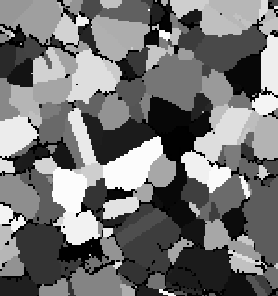
\includegraphics[width=2.5in]{Type1.png}
\caption{}
\label{figure:Type1}
\end{center}
\end{figure}

\begin{figure}[htbp]
\begin{center}

\includegraphics[width=2.5in]{Type2.png}
\caption{}
\label{figure:Type2}
\end{center}
\end{figure}



\begin{figure}[htbp]
\begin{center}
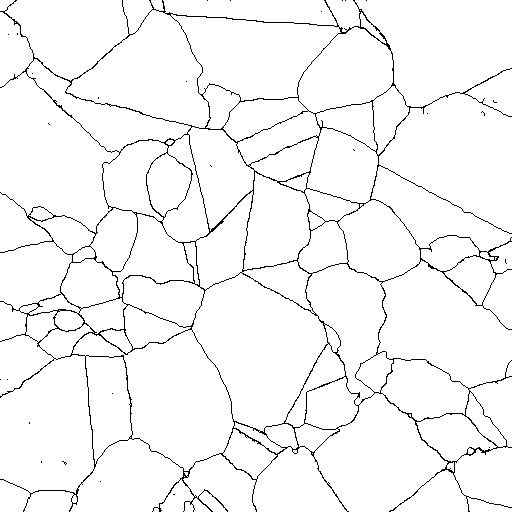
\includegraphics[width=2.5in]{Type3.png}
\caption{}
\label{figure:Type3}
\end{center}
\end{figure}


\end{document}